\documentclass[12pt,a4paper]{article}

% Drake_preamble.tex - LaTeX Preamble Template
% 作者: 謝慕揚, MD, PhD, FESC

% Including essential packages for Chinese typesetting
\usepackage{xeCJK}
\usepackage{fontspec}
% Configuring Chinese font with Noto Serif CJK TC, fallback to SimSun
\IfFontExistsTF{Noto Serif CJK TC}{
  \setCJKmainfont{Noto Serif CJK TC}
  \setCJKsansfont{Noto Serif CJK TC}
  \setCJKmonofont{Noto Serif CJK TC}
}{\setCJKmainfont{SimSun}
  \setCJKsansfont{SimSun}
  \setCJKmonofont{SimSun}
}

% Including other necessary packages
\usepackage{geometry}
\usepackage{titlesec}
\usepackage{enumitem}
\usepackage{xcolor}
\usepackage{colortbl}
\usepackage{tcolorbox}
\usepackage{booktabs}
\usepackage{longtable}
\usepackage{array}
\usepackage{graphicx}
\usepackage{caption}
\usepackage{tikz}
\usepackage{fancyhdr}
\usepackage{multicol}
\usepackage{datetime2}
\usepackage{hyperref}
\usepackage{mdframed}
\usepackage{amsmath}
\usepackage{amssymb}
\usepackage{multirow}

% Defining colors
\definecolor{emergency_red}{RGB}{186,24,27}
\definecolor{emergency_blue}{RGB}{0,114,188}
\definecolor{emergency_gray}{RGB}{120,120,120}
\definecolor{highlight_yellow}{RGB}{255,250,205}

\hypersetup{
    colorlinks=true,
    linkcolor=emergency_blue,
    citecolor=emergency_blue,
    urlcolor=emergency_blue,
    pdfborder={0 0 0}
}

% Defining page geometry
\geometry{
  top=2.5cm,
  bottom=2.5cm,
  left=2cm,
  right=2cm,
  headheight=25pt
}

% Adjusting topmargin to compensate for increased headheight
\addtolength{\topmargin}{-10pt}

% Setting title formats
\titleformat{\section}[block]{\Large\bfseries\color{emergency_red}}{\thesection}{10pt}{}
\titleformat{\subsection}[block]{\large\bfseries\color{emergency_blue}}{\thesubsection}{8pt}{}
\titleformat{\subsubsection}[block]{\normalsize\bfseries\color{emergency_gray}}{\thesubsubsection}{6pt}{}

% Defining custom environment for important notes
\newmdenv[
    linecolor=emergency_red,
    backgroundcolor=highlight_yellow,
    linewidth=2pt,
    topline=true,
    bottomline=true,
    leftline=true,
    rightline=true,
    innertopmargin=10pt,
    innerbottommargin=10pt,
    innerleftmargin=10pt,
    innerrightmargin=10pt
]{importantbox}

% Defining note command with tcolorbox
\newcommand{\note}[1]{
    \par
    \noindent
    \begin{tcolorbox}[
        colback=emergency_blue!5!white,
        colframe=emergency_blue,
        title=\textbf{重點提醒},
        fonttitle=\bfseries,
        boxrule=0.5pt,
        arc=3pt,
        left=6pt,
        right=6pt,
        top=6pt,
        bottom=6pt
    ]
    #1
    \end{tcolorbox}
}

% Key findings box
\newcommand{\keyfinding}[1]{
    \par
    \noindent
    \begin{tcolorbox}[
        colback=yellow!10!white,
        colframe=orange!75!black,
        title=\textbf{核心發現摘要},
        fonttitle=\bfseries,
        boxrule=0.5pt,
        arc=3pt
    ]
    #1
    \end{tcolorbox}
}

% Defining custom date format
\newcommand{\mydate}{\the\year-\the\month-\the\day}

% Custom header
\pagestyle{fancy}
\fancyhf{}
\fancyhead[L]{\textcolor{emergency_red}{周邊血管介入教學講義}}
\fancyhead[R]{\textcolor{emergency_blue}{Persistent Sciatic Artery}}
\fancyfoot[C]{\textcolor{emergency_gray}{\thepage}}
\renewcommand{\headrulewidth}{1pt}
\renewcommand{\headrule}{\hbox to\headwidth{\color{emergency_red}\leaders\hrule height \headrulewidth\hfill}}

\begin{document}

%% Title Page
\begin{center}
{\LARGE\bfseries\textcolor{emergency_red}{周邊血管介入病例討論}}\\[0.5cm]
{\Large\textbf{Persistent Sciatic Artery: A Rare Vascular Anomaly}}\\[0.3cm]
{\large 持續性坐骨動脈：罕見血管變異的診斷與處置}\\[0.5cm]
{\normalsize 新竹台大分院心血管中心病例}\\[0.3cm]
{\normalsize 整理：謝慕揚 MD, PhD, FESC \quad 日期：\mydate}
\end{center}

\vspace{0.5cm}

\keyfinding{
\begin{itemize}[leftmargin=*]
    \item 持續性坐骨動脈 (Persistent Sciatic Artery, PSA) 發生率僅 0.025-0.04\%，極為罕見
    \item 本案為 82 歲女性（MRN: H051516），右側 PSA，介入治療時器械位於 internal iliac artery 內
    \item PSA 動脈瘤發生率高達 48\%，需特別注意血栓栓塞併發症
    \item 診斷關鍵：股動脈搏動減弱但膕動脈搏動正常、Cowie's sign（臀部搏動性腫塊）
    \item 治療策略需根據 Pillet-Gauffre 分類及是否合併動脈瘤決定
\end{itemize}
}

\section{病例呈現}

\subsection{基本資料}

\begin{longtable}{p{4cm}p{10cm}}
\toprule
\textbf{項目} & \textbf{內容} \\
\midrule
\endfirsthead
\bottomrule
\endlastfoot
患者 & 82 歲女性 \\
\midrule
病歷號碼 (MRN) & H051516 \\
\midrule
診斷 & Right-sided Persistent Sciatic Artery \\
\midrule
發現方式 & 周邊血管介入治療時發現 \\
\midrule
關鍵發現 & 介入器械位於 internal iliac artery 內，而非一般的 external iliac $\rightarrow$ femoral artery 路徑 \\
\midrule
操作醫師 & 潘恆宇醫師 \\
\end{longtable}

\subsection{影像學發現}

\begin{figure}[htbp]
\centering
\begin{minipage}{0.48\textwidth}
\centering
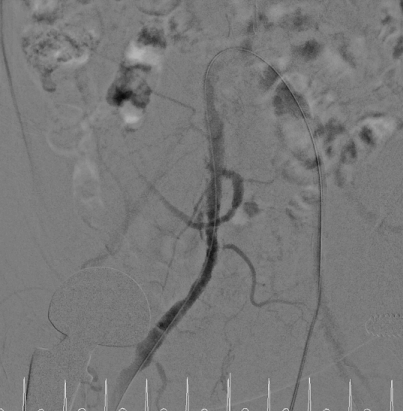
\includegraphics[width=\textwidth]{PSA_angiography.png}
\caption*{\textbf{血管攝影 (Angiography)}\newline 顯示 persistent sciatic artery 走向，介入器械位於 internal iliac artery 內}
\end{minipage}
\hfill
\begin{minipage}{0.48\textwidth}
\centering
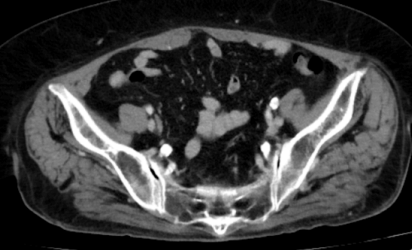
\includegraphics[width=\textwidth]{PSA_CT_axial.png}
\caption*{\textbf{電腦斷層 (CT Axial)}\newline 骨盆腔軸向切面，顯示 PSA 解剖位置}
\end{minipage}
\end{figure}

\begin{importantbox}
\textbf{血管攝影關鍵觀察點}：

從 angiography 不易直接辨識 PSA，需仔細觀察：
\begin{enumerate}
    \item 導管及器械位置：本案器械皆位於 \textbf{internal iliac artery} 內
    \item 正常情況下，下肢介入應經由 external iliac $\rightarrow$ common femoral $\rightarrow$ SFA 路徑
    \item PSA 從 internal iliac artery 延伸，經坐骨大孔至膕動脈
\end{enumerate}
\end{importantbox}

\section{持續性坐骨動脈概述}

\subsection{定義與流行病學}

\begin{itemize}
    \item \textbf{定義}：胚胎發育過程中坐骨動脈未正常退化，持續作為下肢主要血液供應
    \item \textbf{發生率}：0.025-0.04\%（極為罕見）
    \item \textbf{性別分布}：男女比例接近（52.6\% vs 47.4\%）
    \item \textbf{雙側發生率}：約 26.3\%
\end{itemize}

\subsection{胚胎學}

\begin{longtable}{p{4cm}p{10cm}}
\toprule
\textbf{發育階段} & \textbf{說明} \\
\midrule
\endfirsthead
\toprule
\textbf{發育階段} & \textbf{說明} \\
\midrule
\endhead
\bottomrule
\endlastfoot
胚胎早期 & 坐骨動脈是內髂動脈的延續，為下肢芽的主要血液供應 \\
\midrule
胚胎第6-8週 & 股淺動脈 (SFA) 開始發育 \\
\midrule
正常發育 & SFA 與膕動脈建立連續性後，坐骨動脈退化 \\
\midrule
正常殘餘 & 坐骨動脈殘餘形成膕動脈遠端及腓動脈 \\
\midrule
PSA 形成 & 坐骨動脈未退化，持續作為下肢主要血供 \\
\end{longtable}

\subsection{解剖走向}

PSA 從 internal iliac artery 發出，依序經過：
\begin{enumerate}
    \item 梨狀肌 (piriformis muscle) 下方
    \item 坐骨大孔 (greater sciatic foramen)
    \item 沿坐骨神經 (sciatic nerve) 走行
    \item 進入膕窩 (popliteal fossa)
    \item 與膕動脈連續
\end{enumerate}

\note{
\textbf{介入治療重要提示}：由於 PSA 經由 internal iliac artery 供應下肢，介入器械會位於 internal iliac artery 內而非傳統的 external iliac $\rightarrow$ femoral artery 路徑。這是本病例的關鍵發現。
}

\section{Pillet-Gauffre 分類系統}

\subsection{分類說明}

此分類系統由 Pillet (1980) 提出，後由 Gauffre (1994) 修訂。

\begin{longtable}{p{2cm}p{6cm}p{6cm}}
\toprule
\textbf{類型} & \textbf{描述} & \textbf{臨床意義} \\
\midrule
\endfirsthead
\toprule
\textbf{類型} & \textbf{描述} & \textbf{臨床意義} \\
\midrule
\endhead
\bottomrule
\endlastfoot
Type 1 & 完整 PSA + 完整 SFA & 雙重血液供應，風險較低 \\
\midrule
Type 2a & 完整 PSA + 不完整 SFA & \textbf{最常見 (62.5\%)}，需特別注意 \\
\midrule
Type 2b & 完整 PSA + SFA 缺失 & 下肢完全依賴 PSA，高風險 \\
\midrule
Type 3 & 僅 PSA 近端存留 + 正常 SFA & 風險相對較低 \\
\midrule
Type 4 & 僅 PSA 遠端存留 + 正常 SFA & 風險相對較低 \\
\midrule
Type 5a & PSA 起源於中央薦動脈 + 發達 SFA & 變異型 \\
\midrule
Type 5b & PSA 起源於中央薦動脈 + 發育不全 SFA & 需特別注意 \\
\end{longtable}

\subsection{Ahn-Min 新分類與治療建議}

\begin{longtable}{p{2.5cm}p{5cm}p{6.5cm}}
\toprule
\textbf{新分類} & \textbf{對應 Pillet-Gauffre 類型} & \textbf{治療建議} \\
\midrule
\endfirsthead
\bottomrule
\endlastfoot
Class I & Type 1, 5a & 保守治療為主 \\
\midrule
Class II & Type 3, 4 & 視症狀決定 \\
\midrule
Class III & Type 2a, 2b, 5b & 多需手術繞道 \\
\midrule
Class IV & 無法歸類 & 個別化評估 \\
\end{longtable}

\section{臨床表現}

\subsection{症狀分布}

\begin{itemize}
    \item \textbf{無症狀偶然發現}：約 20\%
    \item \textbf{有症狀}：約 80\%
\end{itemize}

\subsection{常見臨床表現}

\begin{longtable}{p{4cm}p{3cm}p{7cm}}
\toprule
\textbf{表現} & \textbf{發生率} & \textbf{說明} \\
\midrule
\endfirsthead
\toprule
\textbf{表現} & \textbf{發生率} & \textbf{說明} \\
\midrule
\endhead
\bottomrule
\endlastfoot
動脈瘤形成 & 25-58\% & 最常見併發症 \\
\midrule
下肢缺血 & 31-63\% & 可能進展至重度缺血 \\
\midrule
間歇性跛行 & 常見 & \textbf{坐姿時加重}（特徵性） \\
\midrule
臀部搏動性腫塊 & 特異性 & Cowie's sign \\
\midrule
坐骨神經症狀 & 可能 & 動脈瘤壓迫神經 \\
\end{longtable}

\subsection{特徵性臨床表現}

\begin{importantbox}
\textbf{Cowie's Sign}
\begin{itemize}
    \item \textbf{定義}：臀部可觸及搏動性腫塊
    \item \textbf{臨床意義}：高度提示 PSA 存在
    \item \textbf{機制}：PSA 經過臀部皮下組織時可被觸及
\end{itemize}

\vspace{0.3cm}

\textbf{坐姿跛行 (Sitting Claudication)}
\begin{itemize}
    \item \textbf{獨特表現}：患者坐下休息時反而出現跛行症狀
    \item \textbf{機制}：髖關節屈曲時，PSA 在梨狀肌與薦棘韌帶之間受壓
    \item \textbf{鑑別重點}：一般動脈阻塞性疾病休息時症狀緩解
\end{itemize}
\end{importantbox}

\subsection{理學檢查要點}

\begin{itemize}
    \item 股動脈搏動減弱或消失
    \item 膕動脈搏動正常（來自 PSA）
    \item 臀部可能觸及搏動性腫塊
    \item 坐姿時下肢症狀可能加重
\end{itemize}

\section{併發症}

\subsection{主要併發症}

\begin{longtable}{p{4cm}p{3cm}p{7cm}}
\toprule
\textbf{併發症} & \textbf{發生率} & \textbf{後果} \\
\midrule
\endfirsthead
\bottomrule
\endlastfoot
動脈瘤 & 48\% & 血栓栓塞、破裂風險 \\
\midrule
血栓栓塞 & 常見 & 急性下肢缺血 \\
\midrule
狹窄 & 7\% & 慢性缺血 \\
\midrule
PSA 阻塞 & 9\% & 嚴重缺血 \\
\midrule
遠端動脈阻塞 & 6\% & 重度肢體缺血 \\
\end{longtable}

\subsection{嚴重後果}

\begin{itemize}
    \item \textbf{重度肢體缺血 (Critical Limb Ischemia)}：高達 25\% 患者
    \item \textbf{截肢率}：8-10\%
    \item \textbf{肢體喪失風險}：有動脈瘤者高達 60\% 可能發生遠端栓塞
\end{itemize}

\note{
由於 PSA 的解剖位置特殊（經過坐骨大孔、沿坐骨神經走行），動脈瘤形成後可能壓迫坐骨神經，造成類似坐骨神經痛的症狀，需與椎間盤疾病鑑別。
}

\section{診斷}

\subsection{影像學檢查}

\begin{longtable}{p{4cm}p{5cm}p{5cm}}
\toprule
\textbf{檢查方式} & \textbf{優點} & \textbf{適應症} \\
\midrule
\endfirsthead
\toprule
\textbf{檢查方式} & \textbf{優點} & \textbf{適應症} \\
\midrule
\endhead
\bottomrule
\endlastfoot
CTA & 首選，全景式成像，可評估解剖變異 & 所有疑似病例 \\
\midrule
MRA & 無輻射，無需碘造影劑 & 顯影劑過敏、腎功能不全 \\
\midrule
DSA & 金標準，可同時介入治療 & 計畫介入治療時 \\
\midrule
都卜勒超音波 & 無創、可重複 & 追蹤監測 \\
\end{longtable}

\subsection{血管攝影診斷要點}

\begin{enumerate}
    \item 下肢血流來自 internal iliac artery 而非 external iliac artery
    \item 股淺動脈可能發育不全或缺失
    \item PSA 經坐骨大孔走行至膕窩
    \item 介入器械位於 internal iliac artery 內（如本病例）
\end{enumerate}

\section{治療}

\subsection{治療原則}

治療策略取決於：
\begin{itemize}
    \item 解剖變異類型（Pillet-Gauffre 分類）
    \item 症狀嚴重程度
    \item 是否有動脈瘤
    \item 髂股動脈系統解剖
\end{itemize}

\subsection{治療選項}

\begin{longtable}{p{5cm}p{9cm}}
\toprule
\textbf{情況} & \textbf{建議治療} \\
\midrule
\endfirsthead
\bottomrule
\endlastfoot
無症狀、無動脈瘤 & 保守觀察 + 定期超音波追蹤 \\
\midrule
有症狀、無動脈瘤 & 藥物治療 $\pm$ 血管成形術 \\
\midrule
有動脈瘤 & 手術繞道 $\pm$ 動脈瘤排除術 \\
\midrule
急性缺血 & 取栓術 $\pm$ 繞道手術 \\
\midrule
Class III/IV & 多需繞道手術 \\
\end{longtable}

\subsection{手術方式}

\begin{enumerate}
    \item \textbf{繞道手術 (Bypass Surgery)}
    \begin{itemize}
        \item 股-膕動脈繞道
        \item 使用自體大隱靜脈或人工血管
    \end{itemize}

    \item \textbf{血管內治療 (Endovascular)}
    \begin{itemize}
        \item 線圈栓塞 (Coil embolization)
        \item 覆膜支架 (Stent graft)
    \end{itemize}

    \item \textbf{混合手術 (Hybrid Procedure)}
    \begin{itemize}
        \item 結合開放手術與血管內治療
    \end{itemize}
\end{enumerate}

\section{學習重點}

\begin{importantbox}
\textbf{Clinical Pearls}

\begin{enumerate}[leftmargin=*]
    \item \textbf{診斷線索}：股動脈搏動減弱但膕動脈搏動正常時，應考慮 PSA

    \item \textbf{Cowie's Sign}：臀部搏動性腫塊高度提示 PSA

    \item \textbf{坐姿跛行}：坐下時症狀加重而非緩解，為 PSA 特徵性表現

    \item \textbf{介入治療}：器械位於 internal iliac artery 內是重要診斷線索

    \item \textbf{動脈瘤風險}：高達 48\%，需定期追蹤

    \item \textbf{雙側檢查}：一側發現 PSA 時，需檢查對側（雙側發生率 26\%）

    \item \textbf{多專科合作}：血管外科、介入放射科、影像診斷專家共同評估
\end{enumerate}
\end{importantbox}

\section{本病例討論}

\begin{itemize}
    \item 本案為 82 歲女性（MRN: H051516），右側 PSA，在周邊血管介入治療時發現
    \item 關鍵發現：介入器械皆位於 internal iliac artery 內
    \item 從血管攝影不易直接辨識，需仔細觀察器械位置
    \item CT 影像可清楚顯示 PSA 的解剖走向
    \item 此病例提醒我們在進行下肢血管介入時，若發現器械位置異常，應考慮血管變異的可能性
\end{itemize}

\section{參考文獻}

\begin{enumerate}
    \item Ahn S, Min SK. Treatment Strategy for Persistent Sciatic Artery and Novel Classification Reflecting Anatomic Status. \href{https://doi.org/10.1016/j.ejvs.2016.05.025}{\textit{Eur J Vasc Endovasc Surg}. 2016;52(3):360-369.}

    \item Kritpracha B, et al. Different Manifestations of Persistent Sciatic Artery and Possible Treatment Options: A Series of Four Cases. \href{https://doi.org/10.3390/diagnostics14212383}{\textit{Diagnostics}. 2024;14(21):2383.}

    \item Bower EB, et al. Persistent sciatic artery: embryology, pathology, and treatment. \textit{J Vasc Surg}. 1993;18(2):242-248.

    \item van Hooft IM, et al. Persistent sciatic artery. \href{https://doi.org/10.1016/j.jvs.2009.07.116}{\textit{J Vasc Surg}. 2010;51(4):1066.}

    \item Paraskevas G, et al. Persistent sciatic artery: a systematic review. \textit{Surg Radiol Anat}. 2015;37(10):1189-1195.
\end{enumerate}

\vspace{1cm}
\begin{center}
\textcolor{emergency_gray}{\rule{0.8\textwidth}{0.5pt}}\\[0.3cm]
\textit{新竹台大分院心血管中心病例討論}\\
病例提供：潘恆宇醫師\\
整理：謝慕揚 MD, PhD, FESC
\end{center}

\end{document}
